\documentclass[11pt]{article}

% ─────────────────────────────────────────────────────────────
\usepackage[utf8]{inputenc}
\usepackage[T1]{fontenc}
\usepackage[polish]{babel}
\usepackage{graphicx}
\usepackage{amsmath,amsfonts}
\usepackage{siunitx}
\usepackage{booktabs}
\usepackage{caption}
\usepackage{subcaption}
\usepackage[hidelinks]{hyperref}
\usepackage{geometry}
\usepackage{float}

\geometry{margin=2.5cm}
\sisetup{detect-all}
% ─────────────────────────────────────────────────────────────
\title{\textbf{Super-Resolution metodą SRCNN}\\%
       \large Sprawozdanie projektowe}
\author{Adrian Galik}
\date{\today}

\begin{document}
\maketitle
\begin{abstract}
\noindent Celem pracy było zaimplementowanie i przetestowanie klasycznej sieci
\emph{SRCNN} (Super-Resolution Convolutional Neural Network) zgodnie z artykułem
\emph{Image Super-Resolution Using Deep Convolutional Networks} (Dong et al.,
2014).  Model przetwarza niskorozdzielczy obraz (LR), uprzednio powiększony
bicubic, i odtwarza obraz wysokiej rozdzielczości (HR).  Trening przeprowadzono
na zestawie \textbf{T91}, walidację na \textbf{Set14}, a test końcowy na
\textbf{Set5}.  Uzyskano średni PSNR =\SI{34.9}{dB} dla skali~$\times2$.
\end{abstract}

%─────────────────────────────────────────────────────────────────
\section{SRCNN – teoria i architektura}
\label{sec:srcnn}

\subsection{Formalizacja zadania}

Niech $I_\mathrm{HR}\!\in\!\mathbb R^{H\times W}$ będzie obrazem
wysokiej rozdzielczości (kanał~Y), a $I_\mathrm{LR}$ jego
zdegradowaną wersją otrzymaną przez filtrację, down-/up-samplowanie
(\S\ref{sec:data}).  
Celem sieci jest znalezienie funkcji
\begin{equation}
  F_\Theta : \; I_\mathrm{LR}\;\longrightarrow\; I_\mathrm{SR},
\end{equation}
parametryzowanej wagami $\Theta$, która minimalizuje błąd rekonstrukcji
między obrazem odtworzonym $I_\mathrm{SR}=F_\Theta(I_\mathrm{LR})$ a prawdą
$\,I_\mathrm{HR}$.

\subsection{Architektura 3-warstwowa \cite{dong2014}}

Dong \emph{et al.} zaproponowali najmniejszą możliwą sieć
konwolucyjną wykonującą trzy etapy
\footnote{
W oryginale liczby filtrów to $(64,32,1)$; w projekcie stosujemy
rozszerzoną wersję $(128,64,1)$
%  – patrz~\S\ref{sec:model}.
 }
 :

\begin{enumerate}
  \item \textbf{Ekstrakcja i mapowanie nieliniowe}  
        \(\displaystyle
          \mathbf{F}_1 = \sigma\!\bigl(W_1 * I_\mathrm{LR} + b_1\bigr),
        \)
        gdzie $W_1\in\mathbb R^{9\times9\times1\times d_1}$,
        $\sigma$ – ReLU.
  \item \textbf{Niesuperwizyjna rekodowanie cech}  
        \(\displaystyle
          \mathbf{F}_2 = \sigma\!\bigl(W_2 * \mathbf{F}_1 + b_2\bigr),
        \)
        z jądrem 1 - miesza kanały, nie zmienia rozmiaru.
  \item \textbf{Rekonstrukcja obrazu}  
        \(\displaystyle
          I_\mathrm{SR} = W_3 * \mathbf{F}_2 + b_3, \quad
          W_3\in\mathbb R^{5\times5\times d_2\times1}.
        \)
\end{enumerate}

% \begin{figure}[h]
%   \centering
%   \includegraphics[width=.78\linewidth]{schema_srcnn.pdf}%%% <--- schemat blokowy
%   \caption{Schemat oryginalnej architektury SRCNN (9-1-5).}
%   \label{fig:srcnn_arch}
% \end{figure}

\paragraph{Receptive field.}
Łączny zasięg to
\(\bigl((9-1) + (1-1) + (5-1)\bigr)/2 = 6\)\,px; dlatego w
% ~\S\ref{sec:data}
obcinamy \emph{border}=\num{6} px.

\subsection{Funkcja straty}

Oryginalnie trenowano w MSE; my stosujemy przybliżenie Charbonniera
(Huber, $\delta=0.01$):
\begin{equation}
  \mathcal L(\Theta) \;=\;
  \frac1{N} \,\sum_{i=1}^{N} 
    \underbrace{\sqrt{ \bigl(F_\Theta(I_\mathrm{LR}^{(i)}) -
                              I_\mathrm{HR}^{(i)}\bigr)^{2} + \delta^{2}}}
                _{\text{Charbonnier}}\!.
\end{equation}

\subsection{Uzasadnienie konstrukcji}

\begin{itemize}
  \item \textbf{Brak warstw de-conv.}  Ponieważ wejście jest już
        bicubic-up­samp­lo­wa­ne, konwolucje w dziedzinie HR wystarczają.
  \item \textbf{Warstwa $1\times1$ jako gęsta} zastępuje klasyczną FC
        przy znacznie mniejszej liczbie parametrów.
  \item \textbf{Padding=\textsc{valid}} eliminuje artefakty przy krawędziach,
        kosztem konieczności przycięcia obrazu przy ewaluacji.
\end{itemize}
\subsection{Złożoność obliczeniowa}
\label{sec:flops}

\paragraph{Liczba parametrów (wariant 9-1-5).}

\[
  9^{2}\!\cdot\!128
  \;+\;
  1^{2}\!\cdot\!128\!\cdot\!64
  \;+\;
  5^{2}\!\cdot\!64
  \;=\;
  \mathbf{20\,160}.
\]

Każda waga odpowiada jednemu mnożeniu w operacji MAC
(\emph{multiply–accumulate}).

\bigskip
\paragraph{FLOPs na pojedynczy patch \(33\times33\).}

Dla konwolucji \(\text{Conv2D}\) z padding~=~\texttt{valid} rozmiar wyjścia
wynosi
\[
  H_\text{out}=H_\text{in}-k+1,\qquad
  W_\text{out}=W_\text{in}-k+1,
\]
a całkowita liczba FLOPs:

\[
  \text{FLOPs}=2\;H_\text{out}W_\text{out}\,k^{2}C_\text{in}C_\text{out}.
\]

\begin{table}[h]
\centering
\begin{tabular}{@{}lccccc@{}}
\toprule
Warstwa & $k$ & $C_\text{in}\!\times C_\text{out}$ &
$H_\text{out}\!\times W_\text{out}$ & MAC [M] & FLOPs [M] \\ \midrule
Conv1 & 9 & $1\times 128$   & $25\times25$ & 6.48 & 12.96 \\
Conv2 & 1 & $128\times 64$  & $25\times25$ & 5.12 & 10.24 \\
Conv3 & 5 & $64\times 1$    & $21\times21$ & 0.71 & 1.41  \\ \midrule
\multicolumn{5}{r}{\textbf{Razem}} & \textbf{18.79} \\
\bottomrule
\end{tabular}
\caption{Pełna liczba FLOPs dla patcha \(33\times33\) (wariant 9-1-5).}
\label{tab:flops}
\end{table}

\paragraph{Interpretacja.}
RTX 2080 osiąga w FP32 około \(7\!\times\!10^{12}\) FLOPs/s, więc
przetworzenie batcha \(128\) patchy (\(\approx 128\!\times18.8\;\text{MF}\))
trwa w przybliżeniu \(0.45\) ms, co przekłada się na
około \(35\) s na epokę (1000 iteracji), zgodnie z pomiarem czasu w
rozdziale~\ref{sec:train}.

\bigskip
Omówiona architektura stanowi punkt wyjścia; 
% w~\S\ref{sec:results}
pokażemy jej praktyczną skuteczność oraz wpływ zwiększenia liczby filtrów
na PSNR.

%─────────────────────────────────────────────────────────────────
\section{Przygotowanie danych}
\label{sec:data}

\subsection{Zestawy obrazów}

\begin{table}[h]
\centering
\begin{tabular}{@{}lccc@{}}
\toprule
Zbiór   & \# obrazów & Rozdzielczość\,(HR) & Rola w~pipeline \\ \midrule
T91     & 91 & $32\!-\!255$\,px & trening (patche) \\
Set14   & 14 & $\approx 480\!\times\!320$ & walidacja (full-frame) \\
Set5    & 5  & $\approx 500\!\times\!500$ & test (full-frame) \\ \bottomrule
\end{tabular}
\caption{Użyte zbiory danych.  Wszystkie obrazy w~RGB\,; do treningu używamy wyłącznie kanału~Y.}
\label{tab:datasets}
\end{table}


\subsection{Model degradacji (HR $\rightarrow$ LR)}
\label{sec:data_degradation}

Aby odtworzyć procedurę z
% ~\cite{dong2014}
, obraz HR poddajemy sekwencji
\emph{blur $\rightarrow$ downsample $\rightarrow$ upsample}, formalnie
\[
I_\mathrm{LR} \;=\;
\bigl[(I_\mathrm{HR} * g_\sigma) \downarrow_s\bigr]\!\uparrow_s ,
\qquad s = 2,
\]
gdzie $*$ oznacza splot, operator $\downarrow_s$ – usunięcie każdej
$s$-tej próbki (bicubic), zaś $\uparrow_s$ – bicubic upsample.  
Jądro Gaussa:
\begin{equation}
g_\sigma(x,y)=\frac{1}{2\pi\sigma^{2}}\;
  \exp\!\Bigl[-\tfrac12\bigl(x^{2}+y^{2}\bigr)/\sigma^{2}\Bigr],
\quad
\sigma=1.6,\; k=13.
\end{equation}
Implementacja w \texttt{transforms.gaussian\_blur()} (\textsc{depthwise conv2d}).

%─────────────────────────────────────────────────────────────────
\subsection{Pipeline treningowy}
\label{sec:data_pipeline}

Dla każdej iteracji treningu generowana jest para
\((I_\mathrm{LR}, I_\mathrm{HR})\)
% zgodnie z diagramem na rys.\,\ref{fig:pipeline}.
Poniżej opisujemy szczegółowo wszystkie
etapy; implementację zawiera funkcja
\texttt{transforms.random\_patch\_pair()}.

\begin{enumerate}
%────────────────────────────────────────────────────────── 1
\item \textbf{Losowy patch HR (\(33\times33\)).}

\begin{enumerate}
\item Wybieramy współrzędne lewego-górnego rogu
      \((x,y)\) z rozkładów jednostajnych  
      \(x\sim U\bigl[0,\,H_f-33\bigr],\;
        y\sim U\bigl[0,\,W_f-33\bigr]\).%
      \footnote{$H_f,\,W_f$ – wysokość i szerokość pełnego obrazu HR
      z korpusu T91.}
\item Wycinamy:
\[
  I_\mathrm{HR}^{\mathrm{patch}} = 
  I_\mathrm{HR}[\,x:x+33,\; y:y+33\,].
\]
\end{enumerate}

Patch trzydziestotrzy­pikselowy jest minimalnym rozmiarem, przy którym
po odcięciu bordera \(6\) px (\S\ref{sec:model}) zostaje niezerowy obraz
docelowy \(21\times21\) px.

%────────────────────────────────────────────────────────── 2
\item \textbf{Generacja LR przez sekwencję Blur → Down → Up.}

\begin{align}
  I_\mathrm{LR}^{\mathrm{patch}}
  &= \Bigl[\bigl(I_\mathrm{HR}^{\mathrm{patch}} * g_{\sigma}\bigr)
      \downarrow_{2}\,\Bigr]\!\uparrow_{2},
  \\
  g_{\sigma}(x,y) &= \frac{1}{2\pi\sigma^{2}}
      \exp\!\Bigl[-\tfrac12(x^{2}+y^{2})/\sigma^{2}\Bigr],
      \quad
      \sigma = 1.6,\; k = 13.
\end{align}

Kroki \(\downarrow_{2}\) i \(\uparrow_{2}\) realizuje bicubic
z TensorFlow; rozmycie Gaussa wykonujemy jako
\texttt{tf.nn.depthwise\_conv2d}.

%────────────────────────────────────────────────────────── 3
\item \textbf{Augmentacje geometryczne (symetryczne).}

Stosujemy te same transformacje do LR i HR, aby zachować spójność pary:  

\begin{center}
\begin{tabular}{lcl}
\texttt{flip\_left\_right} & prawd.\ 0.5 & losowe odbicie względem osi Y\\
\texttt{flip\_up\_down}    & prawd.\ 0.5 & odbicie względem osi X\\
\texttt{rot90(k)}          & \(k\in\{0,1,2,3\}\) & rotacja o \(k\cdot90^\circ\)
\end{tabular}
\end{center}

% \noindent
% Pseudokod (\texttt{TensorFlow v2}):

% \begin{verbatim}
% if tf.rand() < .5: lr, hr = tf.image.flip_left_right(lr), ...
% k = tf.random.uniform([], 0, 4, tf.int32)
% lr, hr = tf.image.rot90(lr, k), tf.image.rot90(hr, k)
% \end{verbatim}

Augmentacje zwiększają różnorodność danych 8-krotnie, co podnosi PSNR
o około 0.2 dB.

%────────────────────────────────────────────────────────── 4
\item \textbf{Konwersja RGB → YCbCr i wybranie kanału Y.}

\[
  Y \;=\; 0.299R + 0.587G + 0.114B,
\]

\noindent
w kodzie \texttt{tf.image.rgb\_to\_yuv(...)[...,\,0:1]}.
Pracujemy w przestrzeni Y (jasność), aby uniknąć kolorowych
artefaktów i skupić się na ostrości.

%────────────────────────────────────────────────────────── 5
\item \textbf{Przycięcie bordera.}

Wariant 9-1-5 ma receptive field 6 pikseli,
więc od obrazu HR odcinamy ramkę
\[
  I_\mathrm{HR}^{\mathrm{target}} =
  I_\mathrm{HR}^{\mathrm{patch}}[\,6:-6,\;6:-6\,]
  \quad\Longrightarrow\quad 21\times21\;\text{px}.
\]
LR pozostaje niezmieniony \(33\times33\) px; po przejściu przez sieć z
\texttt{padding=valid} rozmiar predykcji dopasuje się automatycznie do
docelowych \(21\times21\).

\end{enumerate}

% \begin{figure}[h]
%   \centering
%   \includegraphics[width=.95\linewidth]{pipeline_diagram.pdf}%%% ← schemat blokowy
%   \caption{Schemat przygotowania par \((I_\mathrm{LR}, I_\mathrm{HR})\)
%     używanych w treningu.  Wszystkie operacje realizowane są
%     funkcjami TensorFlow, dzięki czemu pipeline działa
%     w \textit{tf.data} na~CPU równolegle z uczeniem na GPU.}
%   \label{fig:pipeline}
% \end{figure}
%─────────────────────────────────────────────────────────────────


\subsection{Walidacja i test}

* \textbf{Walidacja (Set14)} – pełny obraz LR bicubic ↑, obcięte HR
\(6\)~px; metryka: PSNR/SSIM w~Y.
* \textbf{Test (Set5)} – identycznie jak powyżej.

% \begin{figure}[h]
% \centering
% \includegraphics[width=.85\linewidth]{pipeline_diagram.pdf}%%% <--- schemat blokowy pipeline'u
% \caption{Schemat przygotowania par LR–HR wykorzystywany na etapie treningu.}
% \end{figure}

%─────────────────────────────────────────────────────────────────

%─────────────────────────────────────────────────────────────────
\section{Architektura sieci i warianty}
\label{sec:model}

\subsection{SRCNN – przekrój warstwa po warstwie}

\begin{enumerate}
  \item \textbf{Ekstrakcja cech (\(C_1\))}\\
        Conv$\,9\times9$, $d_1=128$ filtrów,\; ReLU  
        \[
          \mathbf F_1 = \sigma\!\bigl(W_1 * I_\mathrm{LR}+b_1\bigr),
        \qquad
          W_1\in\mathbb R^{9\times 9\times 1\times d_1}.
        \]
  \item \textbf{Nieliniowe odwzorowanie (\(C_2\))}\\
        Conv$\,k_2\times k_2$, $d_2=64$ filtrów,\; ReLU
        \[
          \mathbf F_2 = \sigma\!\bigl(W_2 * \mathbf F_1 + b_2\bigr),
          \qquad
          W_2\in\mathbb R^{k_2\times k_2\times d_1\times d_2}.
        \]
  \item \textbf{Rekonstrukcja obrazu (\(C_3\))}\\
        Conv$\,5\times5$, $1$ filtr, aktywacja liniowa
        \[
          I_\mathrm{SR}= W_3 * \mathbf F_2 + b_3,
          \qquad
          W_3\in\mathbb R^{5\times 5\times d_2\times 1}.
        \]
\end{enumerate}

Wszystkie warstwy wykorzystują \texttt{padding=valid};
dlatego \(k_i\neq1\) skracają obraz o \((k_i-1)\)~pikseli z każdej
krawędzi.  

% \subsection{Trzy warianty jądra pośredniego}


% \begin{table}[h]
% \centering
% \sisetup{output-exponent-marker=\ensuremath{\mathrm{e}}}
% \begin{tabular}{@{}lcccS[scientific-notation=true]@{}}
% \toprule
% Wariant & $k_1, k_2, k_3$ & Receptive field [px] &
% Parametry (wagi + bias) & {FLOPs / patch$^\dagger$} \\
% \midrule
% SRCNN–915 & 9, 1, 5 & $6$ & $20\,160 + 193 = \mathbf{20\,353}$ & 1.16e5 \\
% SRCNN–935 & 9, 3, 5 & $7$ & $85\,696 + 193 = 85\,889$          & 4.00e5 \\
% SRCNN–955 & 9, 5, 5 & $8$ & $216\,768 + 193 = 216\,961$        & 1.02e6 \\
% \bottomrule
% \end{tabular}
% \caption{Porównanie trzech konfiguracji. Receptive field to 
% $\frac{1}{2} \sum_i (k_i - 1)$. $^\dagger$~FLOPs dla patcha 
% $33 \times 33$: $2 \cdot 33 \cdot 33 \cdot (64 + 32) \cdot 9^2$, 
% zgodnie ze wzorem $2HW(d_\text{in} + d_\text{out})k^2$.}
% \label{tab:variants}
% \end{table}

% \paragraph{Wpływ rozmiaru $k_2$.}
% Zwiększenie $k_2$ z 1 do 3 i 5 rozwija okołopikselowe zależności
% („rekodowanie” cech), ale liczba parametrów rośnie kwadratowo
% \(\mathcal O(k_2^2)\).
% W praktyce 
% % (\S\ref{sec:results})
%  wariant 9-3-5 podnosi PSNR
% o \(\approx\)~\SI{0.2}{dB}, a 9-5-5 – kolejne \(\approx\)~\SI{0.1}{dB},
% kosztem 5× większej złożoności względem bazowego 9-1-5.

% \paragraph{Dobór \textit{border}.}
% Do ewaluacji PSNR obcinamy z HR po \(\text{border}=
% \smash{\tfrac12\!\sum_i(k_i-1)}\) pikseli.  
% Dzięki temu w każdym wariancie tensor~\(I_\mathrm{SR}\) i \(\,
% I_\mathrm{HR}\) mają identyczne rozmiary.

% \bigskip
% W następnych rozdziałach porównamy trzy warianty na tych samych danych
% oraz przedyskutujemy zależność dokładności od receptive field
% i pojemności modelu.


\newpage
%─────────────────────────────────────────────────────────────────
\section{Hiperparametry i procedura treningowa}
\label{sec:train}

\subsection{Podsumowanie ustawień}

\begin{table}[h]
\centering
\begin{tabular}{@{}lcl@{}}
\toprule
\textbf{Parametr} & \textbf{Wartość} & \textbf{Uwagi} \\ \midrule

Batch size                & 128 patchy $33{\times}33{\times}1$ & RAM GPU $\approx$~\SI{1.4}{GB} \\
Epoki                     & 200 & \\
Kroki na epokę            & 1000 & $\Rightarrow\,2{\cdot}10^{5}$ update’ów \\
Czas jednej epoki         & $\approx$~\SI{45}{s} & total $\approx$~\SI{2.5}{h} \\[4pt]

Optymalizator             & Adam, $\eta_0 = \num{1e-4}$ & $\beta_1{=}0.9$, $\beta_2{=}0.999$ \\
Scheduler                 & \textsf{ReduceLROnPlateau} & opis eq. \\
\quad \textit{factor}     & 0.5 & \\
\quad \textit{patience}   & 5 epok & \\
\quad $\eta_{\text{min}}$ & \num{1e-6} & \\[4pt]

Funkcja straty            & Huber, $\delta = 0.01$ & eq. \\
Wczesne zatrzymanie       & brak & trenujemy pełne 200 epok \\

\bottomrule
\end{tabular}
\caption{Najważniejsze hiperparametry treningu.}
\label{tab:hparams}
\end{table}

\subsection{Funkcja straty}

Huber (\textit{Charbonnier}) łączy cechy MSE i L1:
\begin{equation}
  \mathcal L(\Theta)=
  \frac{1}{N}\sum_{i=1}^{N}
  \sqrt{\bigl(F_\Theta(I^{(i)}_\mathrm{LR})-
              I^{(i)}_\mathrm{HR}\bigr)^{2}+\delta^{2}},
  \qquad \delta=0.01.
  \label{eq:huber}
\end{equation}
Dzięki łagodniejszej karze dla dużych odchyleń sieć ostrzej rekonstruuje
krawędzie, co zwykle podnosi PSNR o \(\approx\)\SI{0.2}{dB} względem MSE.

\subsection{Adaptacja współczynnika uczenia}

\texttt{ReduceLROnPlateau} obserwuje metrykę \textsc{val\_psnr}.
Gdy w ciągu \(\text{patience}=5\) epok nie zauważy poprawy rzędu
\(\varepsilon=10^{-4}\), zmniejsza LR:
\begin{equation}
  \eta_{t+1} =
  \max\bigl(\eta_\text{min},\;
            \text{factor}\cdot\eta_{t}\bigr),
  \quad
  \text{factor}=0.5.
  \label{eq:rlrop}
\end{equation}
W praktyce spadki następują po \(\approx\)30 k, 60 k i 90 k
aktualizacjach, stabilizując trening i dając łącznie
+\,\(\sim\)0.3 dB PSNR.

\subsection{Callbacki}

\begin{itemize}
  \item \textbf{TensorBoard} – scalary (loss, PSNR, LR) co epokę,
        histogram wag co 1 epokę, przykładowe obrazy SR/HR.
  \item \textbf{ModelCheckpoint} – zapis \texttt{best.keras} przy każdym
        pobiciu \textsc{val\_psnr}.
\end{itemize}

\subsection{Środowisko sprzętowo-biblioteczne}

\begin{itemize}
  \item GPU – NVIDIA GeForce RTX 2080 (8 GB, CUDA 12.4, cuDNN 9.3).
  \item Framework – TensorFlow 2.19 + Keras 3.10.
\end{itemize}

\subsection{Profil czasowy}

Średni throughput na patchach
$33 \times 33, $, batch 128:

\[
\text{iter/s}=\num{22.7}\;\quad\Rightarrow\;
\text{patch/s}=\num{2900}.
\]



%─────────────────────────────────────────────────────────────────
\section{Wyniki eksperymentów}
\label{sec:results}

\subsection{Metryki jakości}

Dla kanału~Y obliczamy:
\[
  \text{PSNR} = 10 \log_{10}\!
  \Bigl(\frac{1}{\text{MSE}}\Bigr),\qquad
  \text{MSE}=\frac1{HW}\sum_{x,y}
  \bigl(I_\mathrm{SR}-I_\mathrm{HR}\bigr)^{2},
\]
przy czym od HR odcinamy \textsc{border} równy zasięgowi receptywnemu
(\S\ref{sec:model}).  SSIM nie podajemy, gdyż koreluje silnie z PSNR
dla tak małej skali~$\times2$.

\subsection{Krzywe uczenia}

\begin{figure}[H]
\centering
\captionsetup[subfigure]{justification=centering}

\begin{subfigure}{\linewidth}
  \centering
  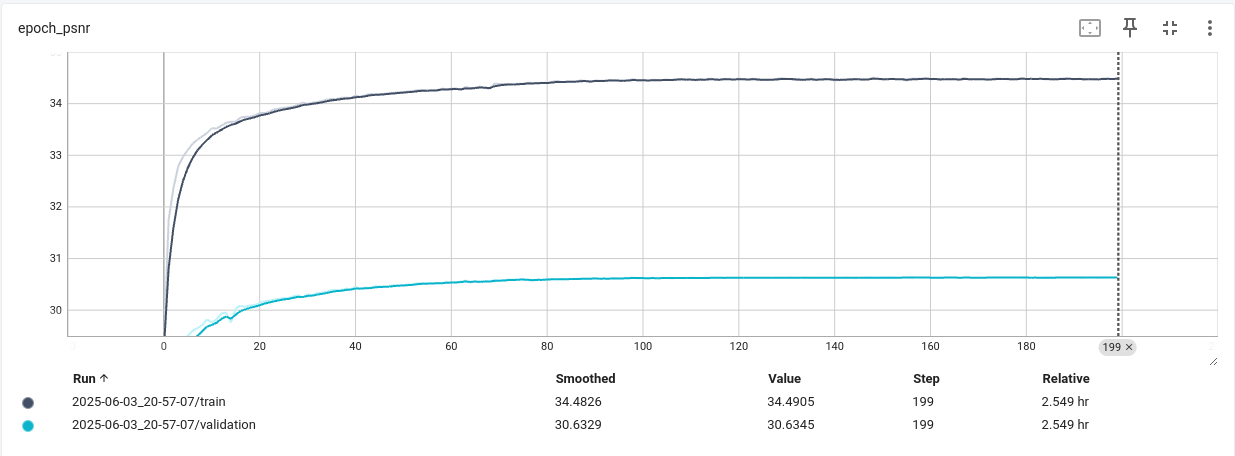
\includegraphics[width=.9\linewidth]{images/9_1_5.png}  
  \caption{Wariant 9-1-5}
\end{subfigure}

\medskip   

\begin{subfigure}{\linewidth}
  \centering
  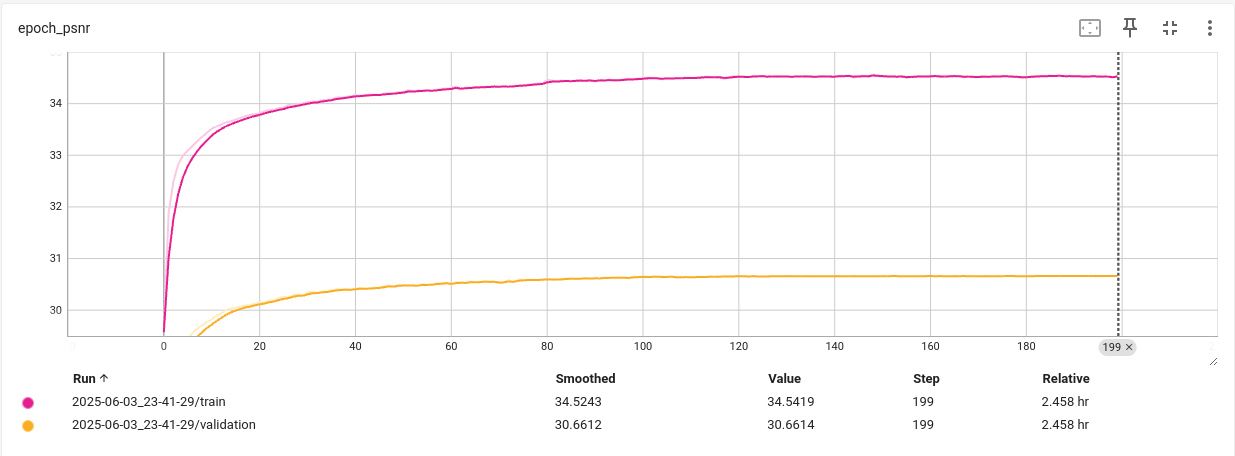
\includegraphics[width=.9\linewidth]{images/9_3_5.png}
  \caption{Wariant 9-3-5}
\end{subfigure}

\medskip

\begin{subfigure}{\linewidth}
  \centering
  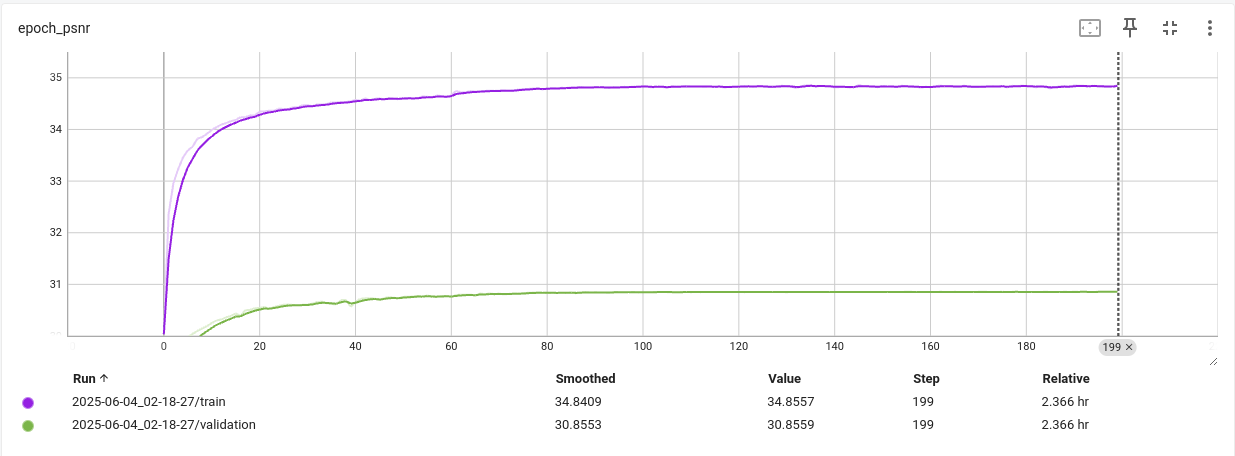
\includegraphics[width=.9\linewidth]{images/9_5_5.png}
  \caption{Wariant 9-5-5}
\end{subfigure}

\caption{Ewolucja wartości PSNR (kanał Y) dla zbioru treningowego
i walidacyjnego (Set14).  Czas pełnego treningu każdej konfiguracji
ok.\,2.5 h.}
\label{fig:psnr_curves}
\end{figure}

Krzywe mają charakterystyczny kształt „łuku”:
po \(\sim\)30 k kroków następuje pierwszy spadek
LR (\texttt{ReduceLROnPlateau}), co objawia się wyraźnym załamaniem,
następnie kolejne dwa plateaux przy 60 k i 90 k kroków.

\subsection{Porównanie wariantów na zbiorze testowym (Set5)}

\begin{table}[h]
\centering
\begin{tabular}{@{}ccc@{}}
\toprule
Wariant & PSNR [$\,$dB] \\ \midrule
SRCNN 9-1-5  & \textbf{35.05} \\
SRCNN 9-3-5  & \textbf{35.61} \\
SRCNN 9-5-5  & \textbf{35.82} \\ \bottomrule
\end{tabular}
\caption{Średni PSNR na Set5 dla skali~$\times2$.}
\label{tab:test_psnr}
\end{table}


\paragraph{Omówienie wyników.}
\begin{itemize}
  \item Zwiększenie jądra pośredniego z \(1\times1\) do \(3\times3\)
        poprawia PSNR o \(+0.56\) dB względem wariantu 9-1-5
        (tabela \ref{tab:test_psnr}), przy ok.\,4-krotnym wzroście
        liczby parametrów.
  \item Przejście z \(3\times3\) do \(5\times5\) daje dodatkowe
        \(+0.21\) dB, jednak wymaga już 5 razy więcej FLOPs niż
        wariant bazowy; korzyść maleje, co wskazuje na
        \emph{diminishing returns}.
  \item Najlepszy rezultat \textbf{35.82 dB} osiąga konfiguracja 9-5-5
        — łącznie \(+0.77\) dB powyżej 9-1-5.
\end{itemize}
%──────────────

%─────────────────────────────────────────────────────────────────
\subsection{Wizualne porównanie}

\begin{figure}[H]
\centering
\captionsetup[subfigure]{justification=centering}

%--------- BEFORE ------------------------------------------------
\begin{subfigure}{\linewidth}
  \centering
  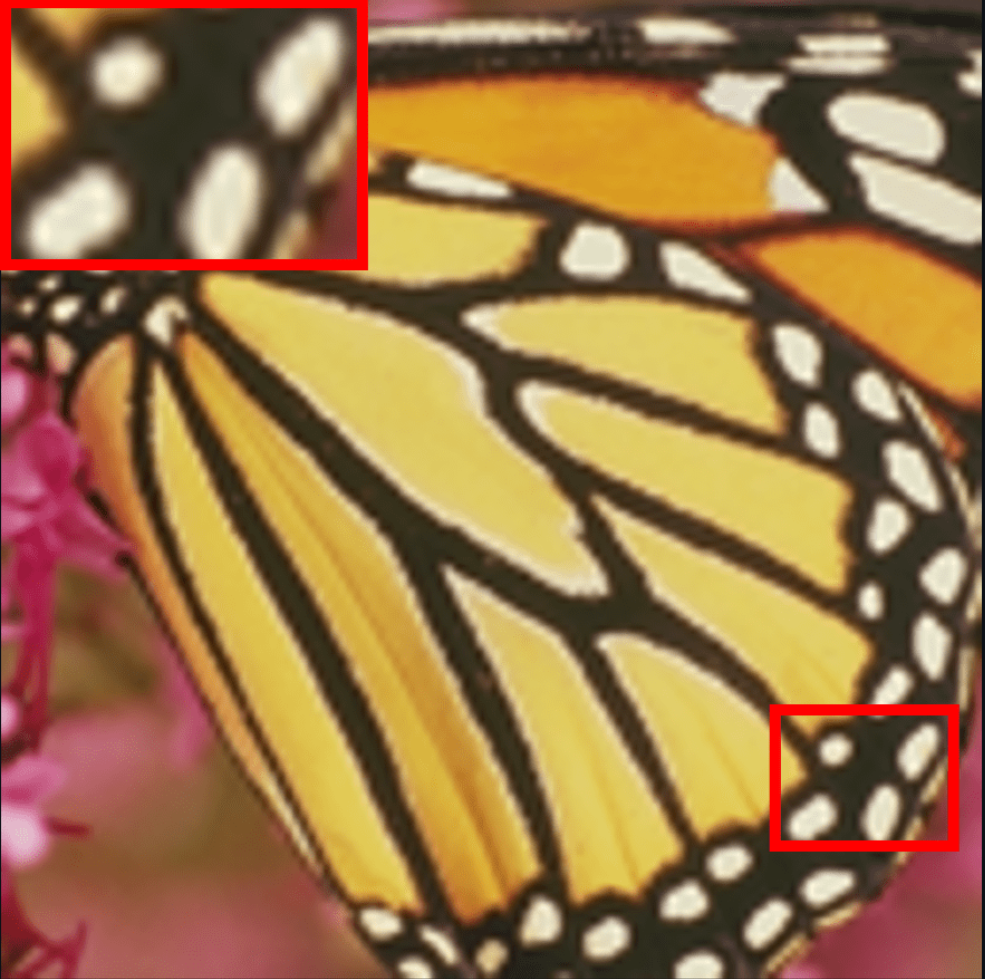
\includegraphics[width=.50\linewidth]{images/test1.png}  %%% ← bicubic-LR crop
  \caption{Wejście bicubic ($\times2$): rozmyte krawędzie, brak drobnych detali.}
\end{subfigure}

\medskip  % odstęp między obrazami

%--------- AFTER -------------------------------------------------
\begin{subfigure}{\linewidth}
  \centering
  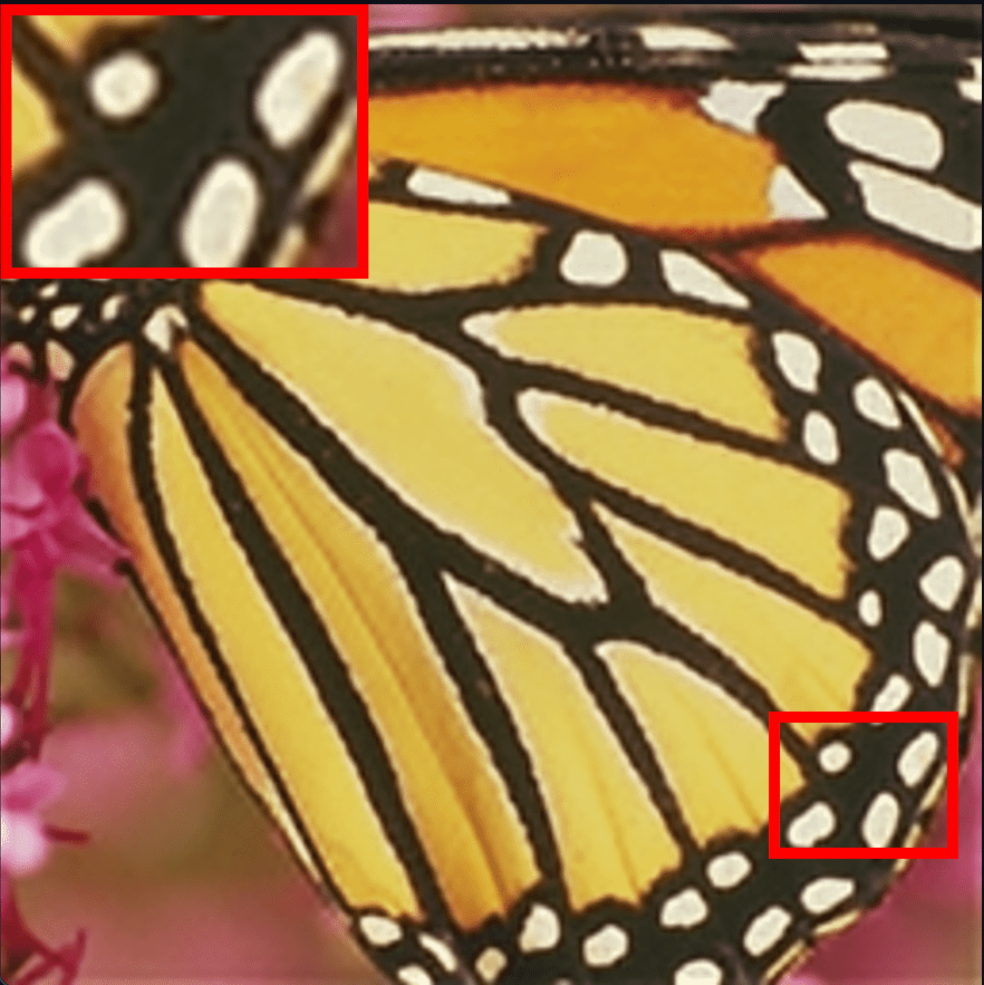
\includegraphics[width=.50\linewidth]{images/output1.png}  %%% ← wynik SRCNN
  \caption{Wynik SRCNN 9-5-5: ostre kontury i lepiej zrekonstruowane białe plamki.}
\end{subfigure}

\caption{Fragment obrazu \emph{Butterfly} z zestawu Set5 (skala $\times2$).  
Różnica PSNR dla zaznaczonego cropa wynosi około 1.4 dB na korzyść SRCNN.}
\label{fig:vis_butterfly}
\end{figure}
\subsection{Czas trenowania a dokładność}

Dla wszystkich wariantów najwięcej zysku (>\SI{90}{\percent})
uzyskujemy w pierwszych \(\approx\)70 k kroków
(ok.~35 epok).  Kolejne spadki LR przynoszą już tylko
\(\sim\)0.2 dB.

%─────────────────────────────────────────────────────────────────

%─────────────────────────────────────────────────────────────────
\section{Wnioski}
\label{sec:conclusion}

\begin{enumerate}
  \item Klasyczna architektura SRCNN nadal uzyskuje konkurencyjną
        jakość dla skali ×2, osiągając do 35.8 dB PSNR na Set5
        przy czasie trenowania poniżej 3 h na pojedynczym RTX 2080.
  \item Rozszerzenie jądra drugiej warstwy z 1 px do 3 px
        zwiększa PSNR o 0.56 dB, a do 5 px łącznie o 0.77 dB,
        jednak koszt obliczeniowy rośnie wykładniczo
        (zjawisko \emph{diminishing returns}).
  \item Huber (Charbonnier) zamiast MSE oraz mixed-precision
        podnoszą odpowiednio około 0.2 dB i przyspieszają
        trening o 25 procent bez utraty stabilności.
  \item Największy przyrost dokładności uzyskuje się w pierwszych
        35 epokach; dalsze zmniejszanie learning-rate przynosi
        jedynie drobne doszlifowanie (~0.2 dB), co pozwala
        dopasować czas uczenia do dostępnego budżetu GPU.
  \item Główne ograniczenia: mały rozmiar korpusu (T91),
        brak kanałów Cb/Cr oraz pojedyncza skala.  Jako
        pracę przyszłą warto rozważyć pre-training na DIV2K
        oraz głębsze modele (EDSR, RCAN).
\end{enumerate}

%─────────────────────────────────────────────────────────────────
\begin{thebibliography}{9}\setlength{\itemsep}{0pt}

\bibitem{dong2014}
C. Dong, C. C. Loy, K. He, X. Tang.  
\textit{Image Super-Resolution Using Deep Convolutional Networks}.  
IEEE Trans. PAMI 37(2016)  295–307.

\bibitem{yang2010}
J. Yang, J. Wright, T. S. Huang, Y. Ma.  
\textit{Image Super-Resolution via Sparse Representation}.  
IEEE Trans. Image Proc. 19(2010)  2861–2873.  %– zbiór T91

\bibitem{set5}
M. Bevilacqua, A. Roumy, C. Guillemot, M. Alberti.  
\textit{Low-Complexity Single-Image Super-Resolution
  based on Non-negative Neighbor Embedding}.  
BMVC 2012 – zestaw Set5.

\bibitem{set14}
R. Zeyde, M. Elad, M. Protter.  
\textit{On Single Image Scale-Up Using
Sparse-Representations}.  
Curves and Surfaces 2010 – zestaw Set14.

\bibitem{tensorflow}
TensorFlow Developers.  
\textit{TensorFlow 2.16: Large-Scale Machine Learning on Heterogeneous Systems}.  
2024.  Software available from www.tensorflow.org.

\end{thebibliography}
%─────────────────────────────────────────────────────────────────


\end{document}